% Options for packages loaded elsewhere
\PassOptionsToPackage{unicode}{hyperref}
\PassOptionsToPackage{hyphens}{url}
%
\documentclass[
]{article}
\usepackage{amsmath,amssymb}
\usepackage{iftex}
\ifPDFTeX
  \usepackage[T1]{fontenc}
  \usepackage[utf8]{inputenc}
  \usepackage{textcomp} % provide euro and other symbols
\else % if luatex or xetex
  \usepackage{unicode-math} % this also loads fontspec
  \defaultfontfeatures{Scale=MatchLowercase}
  \defaultfontfeatures[\rmfamily]{Ligatures=TeX,Scale=1}
\fi
\usepackage{lmodern}
\ifPDFTeX\else
  % xetex/luatex font selection
    \setmainfont[]{lmodern}
\fi
% Use upquote if available, for straight quotes in verbatim environments
\IfFileExists{upquote.sty}{\usepackage{upquote}}{}
\IfFileExists{microtype.sty}{% use microtype if available
  \usepackage[]{microtype}
  \UseMicrotypeSet[protrusion]{basicmath} % disable protrusion for tt fonts
}{}
\makeatletter
\@ifundefined{KOMAClassName}{% if non-KOMA class
  \IfFileExists{parskip.sty}{%
    \usepackage{parskip}
  }{% else
    \setlength{\parindent}{0pt}
    \setlength{\parskip}{6pt plus 2pt minus 1pt}}
}{% if KOMA class
  \KOMAoptions{parskip=half}}
\makeatother
\usepackage{xcolor}
\usepackage[margin=1in]{geometry}
\usepackage{graphicx}
\makeatletter
\def\maxwidth{\ifdim\Gin@nat@width>\linewidth\linewidth\else\Gin@nat@width\fi}
\def\maxheight{\ifdim\Gin@nat@height>\textheight\textheight\else\Gin@nat@height\fi}
\makeatother
% Scale images if necessary, so that they will not overflow the page
% margins by default, and it is still possible to overwrite the defaults
% using explicit options in \includegraphics[width, height, ...]{}
\setkeys{Gin}{width=\maxwidth,height=\maxheight,keepaspectratio}
% Set default figure placement to htbp
\makeatletter
\def\fps@figure{htbp}
\makeatother
\setlength{\emergencystretch}{3em} % prevent overfull lines
\providecommand{\tightlist}{%
  \setlength{\itemsep}{0pt}\setlength{\parskip}{0pt}}
\setcounter{secnumdepth}{5}
\usepackage{mathpazo}
\usepackage{tabularx}
\usepackage{booktabs}
\renewcommand{\contentsname}{Sumário}
\AtBeginDocument{\fontsize{12}{14}\selectfont}
\usepackage{indentfirst}
\setlength{\parindent}{1.5em}
\usepackage{booktabs}
\usepackage{subcaption}
\usepackage[utf8]{inputenc}
\usepackage[T1]{fontenc}
\usepackage{booktabs}
\usepackage{longtable}
\usepackage{array}
\usepackage{multirow}
\usepackage{wrapfig}
\usepackage{float}
\usepackage{colortbl}
\usepackage{pdflscape}
\usepackage{tabu}
\usepackage{threeparttable}
\usepackage{threeparttablex}
\usepackage[normalem]{ulem}
\usepackage{makecell}
\usepackage{xcolor}
\ifLuaTeX
  \usepackage{selnolig}  % disable illegal ligatures
\fi
\usepackage{bookmark}
\IfFileExists{xurl.sty}{\usepackage{xurl}}{} % add URL line breaks if available
\urlstyle{same}
\hypersetup{
  pdftitle={Séries Temporais dos Acessos à Página do Flamengo na Wikipédia em Português},
  pdfauthor={JJ},
  hidelinks,
  pdfcreator={LaTeX via pandoc}}

\title{Séries Temporais dos Acessos à Página do Flamengo na Wikipédia em
Português}
\author{JJ}
\date{}

\begin{document}
\maketitle

{
\setcounter{tocdepth}{2}
\tableofcontents
}
\newpage

\section{Descrição da base de
dados}\label{descriuxe7uxe3o-da-base-de-dados}

Os dados analisados neste trabalho foram extraídos da base WikiMedia,
que registra o número de acessos diários e mensais a páginas da
Wikipédia. Para este estudo, foi selecionada a página do \textbf{Clube
de Regatas do Flamengo}, considerando exclusivamente acessos humanos,
não automatizados e provenientes de todas as plataformas (desktop,
mobile, etc.).

O período analisado abrange de julho de 2015 (2015-07) a abril de 2025
(2025-04).

\begin{table}[ht]
  \setlength\tabcolsep{12pt}               % espaço interno nas células
  \renewcommand{\arraystretch}{1.2}        % altura das linhas
  \centering
  \caption{Amostra dos dados de acessos à página do Flamengo na Wikipédia}
  \begin{tabularx}{\textwidth}{@{} l >{\raggedleft\arraybackslash}X @{}}
    \toprule
    Data       & Acessos   \\
    \midrule
    2015-07-01 &  69\,072  \\
    2015-08-01 &  69\,949  \\
    2015-09-01 &  61\,722  \\
    2015-10-01 &  40\,512  \\
    2015-11-01 &  45\,647  \\
    2015-12-01 &  57\,336  \\
    \bottomrule
    \multicolumn{2}{@{}l}{\footnotesize Fonte: WikiMedia; dados filtrados para acessos humanos de todas as plataformas.}
  \end{tabularx}
\end{table}

\section{\texorpdfstring{\textbf{Pré-processamento}}{Pré-processamento}}\label{pruxe9-processamento}

A análise visual da série indica que há sazonalidade e que há suspeita
de não estacionariedade. Fora isso, também podemos observar a presença
de um grande outlier.

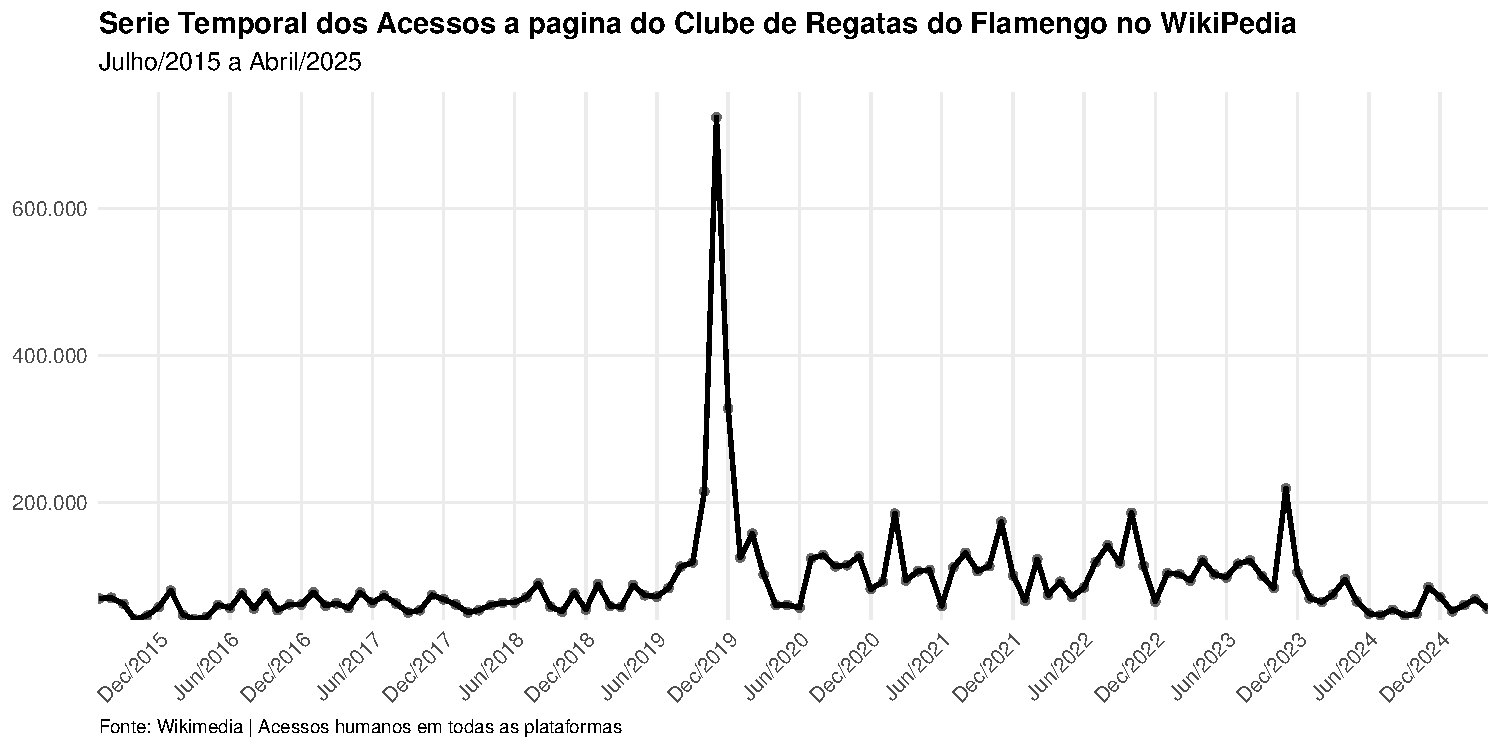
\includegraphics{analise-series-temporais-flamengo_files/figure-latex/unnamed-chunk-3-1.pdf}

\newpage

Primeiramente, iremos nos preocupar com os outliers e, para isso, será
usada a função \emph{tso} para identificá-los e iremos retirar usando a
função \emph{na.approx} que faz, automaticamente, interpolação linear
nas entradas escolhidas (se houver outliers nas extremidades,
utilizaremos o valor mais próximo).

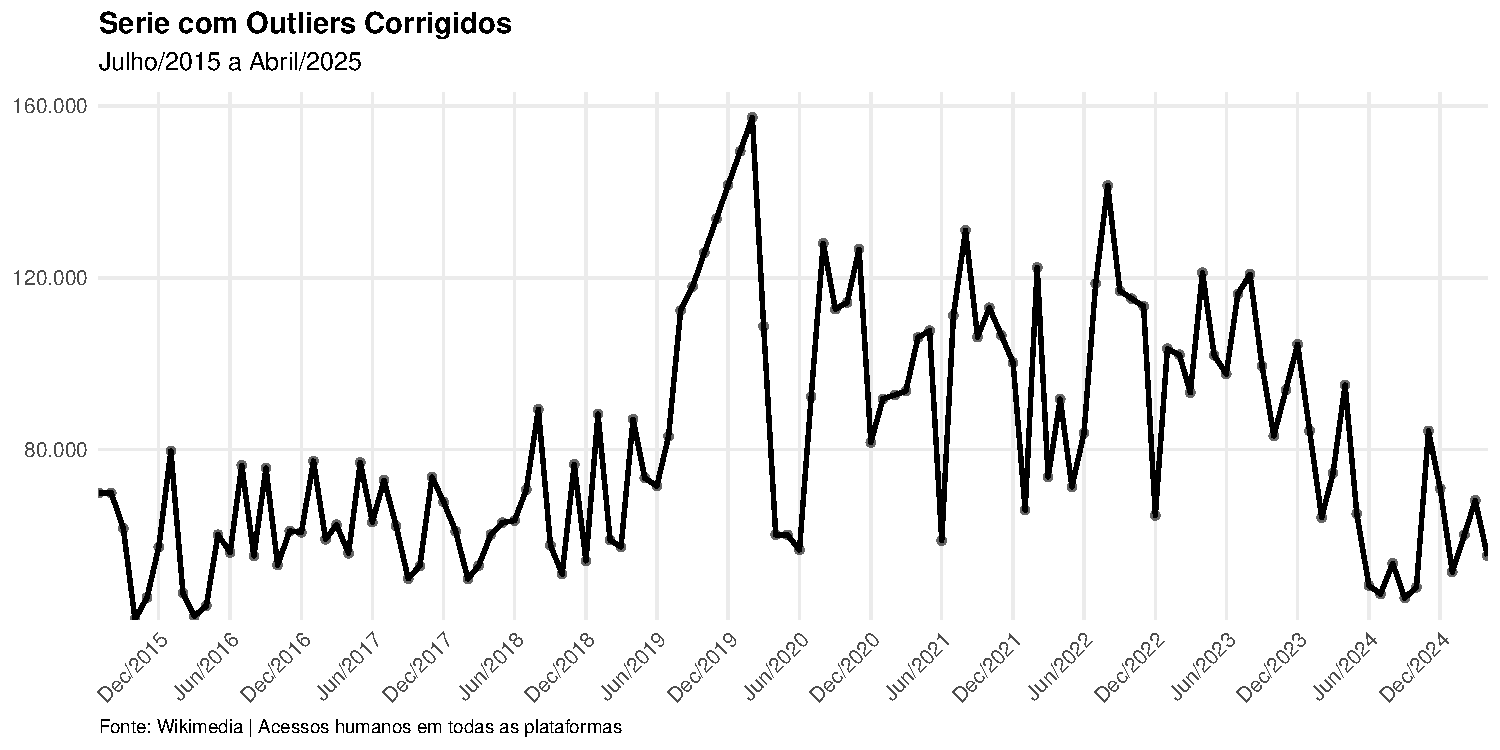
\includegraphics{analise-series-temporais-flamengo_files/figure-latex/unnamed-chunk-4-1.pdf}

Agora, já com os outliers retirados, iremos retirar a sazonalidade
usando a função \emph{STL} que ajusta modelos de regressões locais para
cada janela de um ano, extraindo o padrão médio de repetição. Assim,
identificando o componente sazonal, será usada a função \emph{seasadj}
para obter a série ajustada sem a componente.

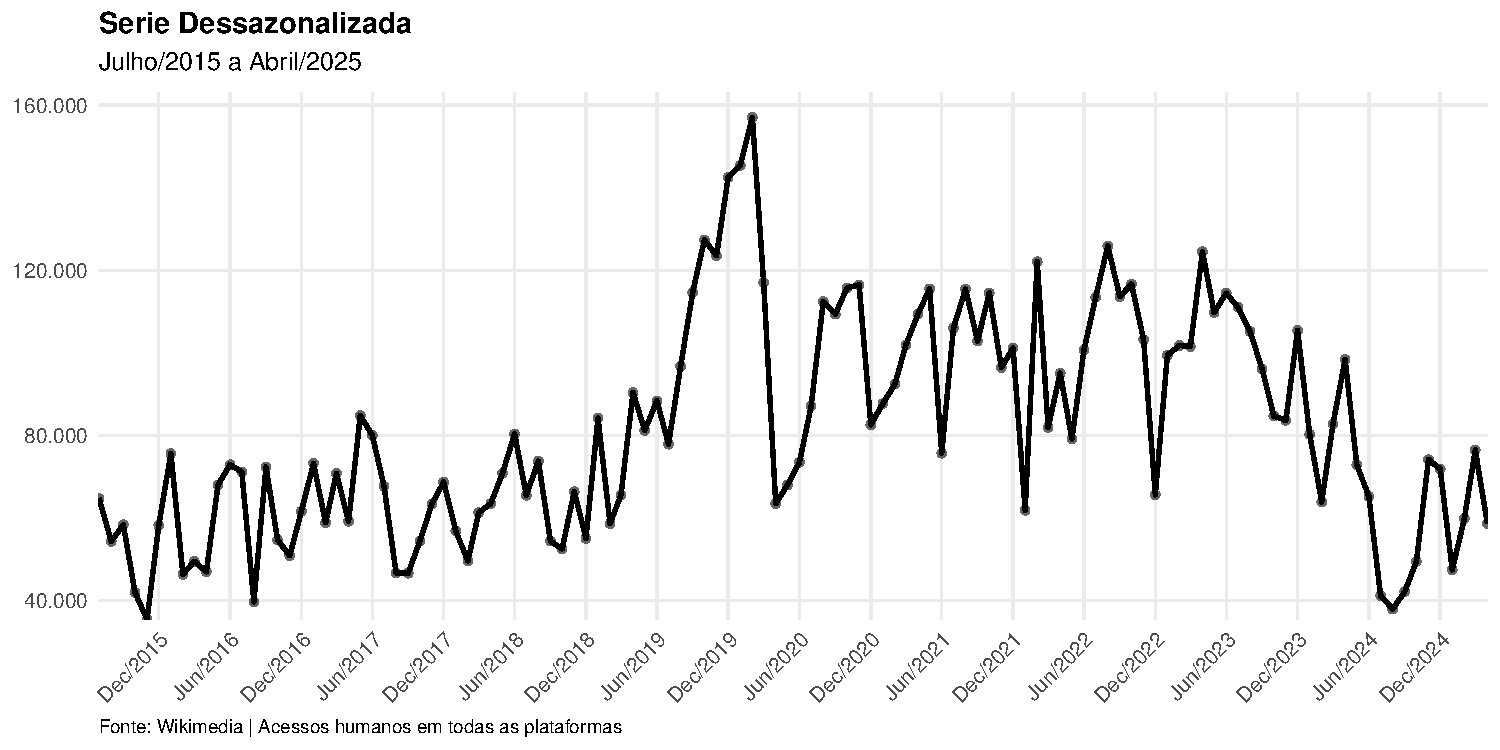
\includegraphics{analise-series-temporais-flamengo_files/figure-latex/unnamed-chunk-5-1.pdf}

\newpage

Agora, já tendo a série dessazonalizada, iremos conferir a outra
suspeita inicial, que a série poderia não ser estacionária.

Para isso, faremos o teste ADF, que confere se a série é estacionária ou
não. Nele, a hipótese alternativa (H1) é: ``a série é estacionária''.

\begin{table}[!h]
\centering
\caption{\label{tab:tab:adf}Resultado do Teste ADF}
\centering
\begin{tabular}[t]{rrl}
\toprule
Estatistica & p\_valor & Hipotese\_Alternativa\\
\midrule
-2.2015 & 0.4929 & stationary\\
\bottomrule
\end{tabular}
\end{table}

O valor do teste foi de -2.2015, com um p-valor de 0.4929. Esse
resultado indica que a hipótese nula de não estacionariedade não pode
ser rejeitada ao nível de significância de 5\%. Ou seja, não há
evidências para concluir que a série é estacionária. Assim, a série pode
apresentar tendência ou dependência temporal de longo prazo, sendo
necessária, então, a diferenciação do modelo.

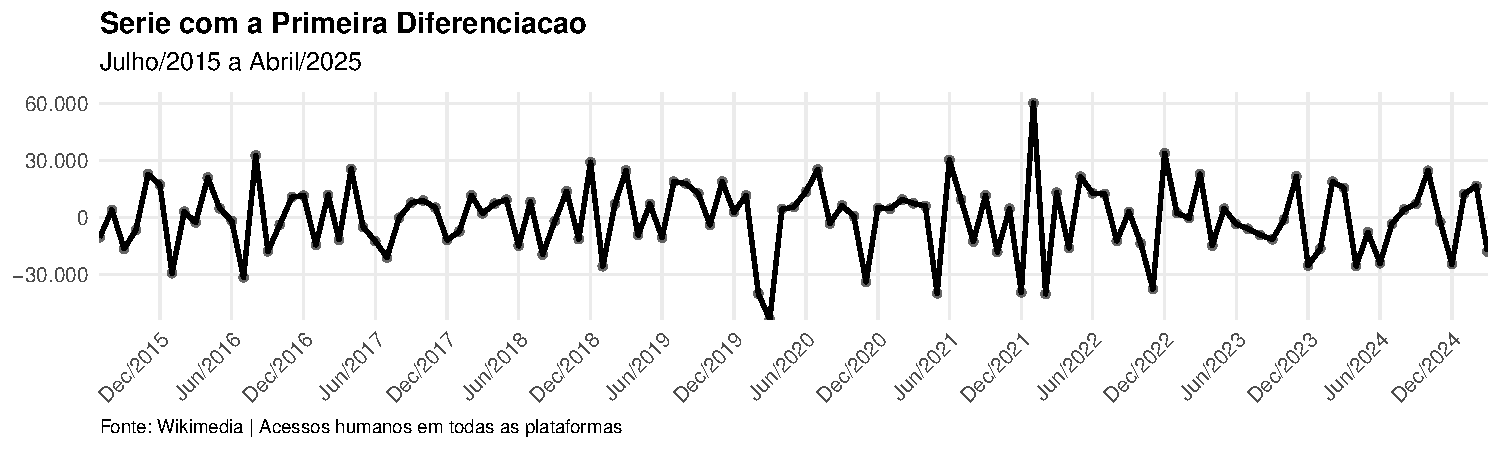
\includegraphics{analise-series-temporais-flamengo_files/figure-latex/unnamed-chunk-7-1.pdf}

Agora a série está no formato ideal e com as características necessárias
para nossas análises, identificações e estimações.

Para avaliar se os modelos conseguem prever bem os dados futuros, a
série temporal foi dividida em duas partes: treino e teste. A parte de
treino vai de julho de 2015 até abril de 2023, e foi usada para ajustar
os modelos. Já o período de teste, de maio de 2023 a abril de 2025, foi
separado para verificar se as previsões realmente funcionam em dados que
o modelo ainda não viu.

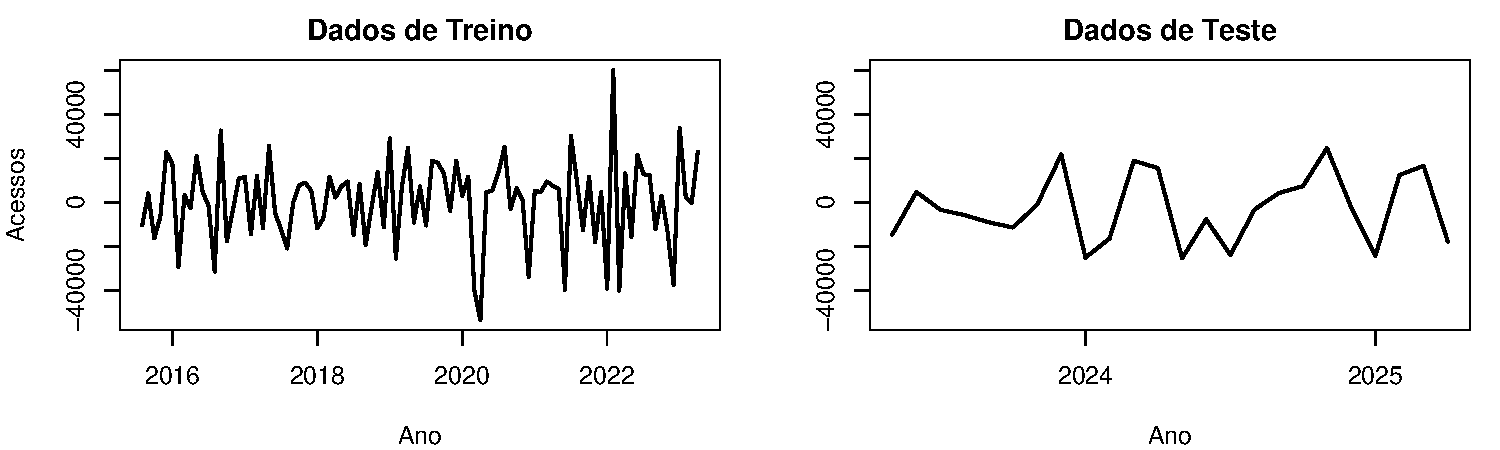
\includegraphics{analise-series-temporais-flamengo_files/figure-latex/unnamed-chunk-8-1.pdf}

\newpage

\section{\texorpdfstring{\textbf{Identificação do Modelo com Base na FAC
e
FACP}}{Identificação do Modelo com Base na FAC e FACP}}\label{identificauxe7uxe3o-do-modelo-com-base-na-fac-e-facp}

Para a identificação da estrutura do modelo, será considerada apenas a
porção de treino da série, composta pelos dados de julho de 2015 a abril
de 2023. A análise se baseia nas funções de autocorrelação (FAC) e
autocorrelação parcial (FACP), aplicadas sobre a série já diferenciada.
A partir da interpretação desses gráficos, será proposto um modelo
inicial, que servirá como base para o resto do trabalho.

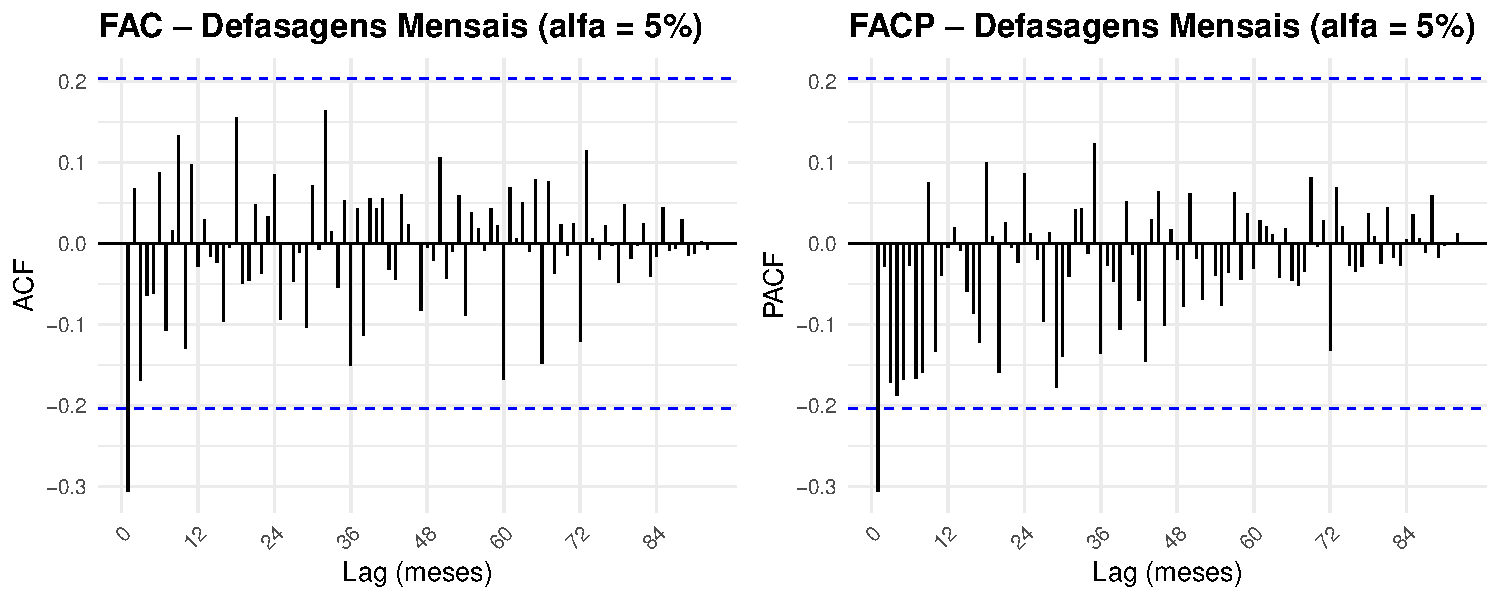
\includegraphics{analise-series-temporais-flamengo_files/figure-latex/acf-pacf-1.pdf}

Em ambos os gráficos se pode observar truncamento no \emph{lag 1}, o que
fornece para nós a sugestão de um modelo inicial \textbf{ARIMA(1,1,1)},
ou \textbf{ARMA(1,1)} considerando que a gente já fez a diferenciação
nos dados. Portanto, iremos começar a nossa análise com a ideia de que,
pela \emph{FAC} e \emph{FACP}, temos um modelo \textbf{ARMA(1,1)}, com a
seguinte equação:

\begin{equation}
X_t = \phi_1 X_{t-1} + \varepsilon_t + \theta_1 \varepsilon_{t-1}, \quad \varepsilon_t \sim \text{N}(0, \sigma^2)
\end{equation}

\section{\texorpdfstring{\textbf{Sobrefixação e estimação do
modelo}}{Sobrefixação e estimação do modelo}}\label{sobrefixauxe7uxe3o-e-estimauxe7uxe3o-do-modelo}

Na última seção, vimos que pela FAC e FACP escolhemos um modelo
\textbf{ARMA(1,1)}. Nesta parte, iremos avaliar o modelo escolhido,
fazer sobrefixação para tentar encontrar o melhor modelo e depois
estimar os parâmetro.

Para isso, consideraremos os seguintes modelos candidatos:
\textbf{ARMA(1,1)}, \textbf{ARMA(2,1)}, \textbf{ARMA(1,2)} e
\textbf{ARMA(2,2)}. Em seguida, faremos a comparação entre eles, a fim
de escolher o modelo final mais adequado para a série em questão.

\newpage

\begin{table}[!ht]
  \centering
  \caption{Coeficientes e testes-z dos modelos ARMA}
  \label{tab:coef_arma}
  \begin{subtable}[t]{0.45\textwidth}
    \centering
    \caption{ARMA(1,1)}
    \begin{tabular}{lrrrr}
      \toprule
      Termo & Estimate & Std.\ Error & z value & Pr(>|z|)\\
      \midrule
      ar1 & -0.5457 & 0.0877 & -6.2192 & 0.0000\textsuperscript{***}\\
      ma1 & -1.0000 & 0.0277 & -36.0502 & 0.0000\textsuperscript{***}\\
      \bottomrule
    \end{tabular}
  \end{subtable}%
  \hfill
  \begin{subtable}[t]{0.45\textwidth}
    \centering
    \caption{ARMA(2,1)}
    \begin{tabular}{lrrrr}
      \toprule
      Termo & Estimate & Std.\ Error & z value & Pr(>|z|)\\
      \midrule
      ar1 & -0.7101 & 0.1012 & -7.0181 & 0.0000\textsuperscript{***}\\
      ar2 & -0.2908 & 0.1006 & -2.8897 & 0.0038\textsuperscript{**}\\
      ma1 & -1.0000 & 0.0281 & -35.6408 & 0.0000\textsuperscript{***}\\
      \bottomrule
    \end{tabular}
  \end{subtable}

  \medskip

  \begin{subtable}[t]{0.45\textwidth}
    \centering
    \caption{ARMA(1,2)}
    \begin{tabular}{lrrrr}
      \toprule
      Termo & Estimate & Std.\ Error & z value & Pr(>|z|)\\
      \midrule
      ar1 & -0.1322 & 0.1056 & -1.2512 & 0.2109\\
      ma1 & -1.9967 & 0.0472 & -42.3056 & 0.0000\textsuperscript{***}\\
      ma2 &  0.9996 & 0.0471 & 21.2189 & 0.0000\textsuperscript{***}\\
      \bottomrule
    \end{tabular}
  \end{subtable}%
  \hfill
  \begin{subtable}[t]{0.45\textwidth}
    \centering
    \caption{ARMA(2,2)}
    \begin{tabular}{lrrrr}
      \toprule
      Termo & Estimate & Std.\ Error & z value & Pr(>|z|)\\
      \midrule
      ar1 & -0.1376 & 0.1070 & -1.2856 & 0.1986\\
      ar2 & -0.0294 & 0.1065 & -0.2762 & 0.7824\\
      ma1 & -1.9970 & 0.0478 & -41.7859 & 0.0000\textsuperscript{***}\\
      ma2 &  0.9999 & 0.0477 & 20.9559 & 0.0000\textsuperscript{***}\\
      \bottomrule
    \end{tabular}
  \end{subtable}
\end{table}

\begin{table}[!h]
  \centering
  \caption{Comparacao de AIC e BIC entre os modelos ajustados}
  \label{tab:criterios_arma}
  \begin{tabular}{lrrr}
    \toprule
    Modelo    &     AIC    &     BIC    \\
    \midrule
    ARMA(1,2) & 2060.995 & 2071.038 \\
    ARMA(2,2) & 2062.918 & 2075.472 \\
    ARMA(2,1) & 2088.374 & 2098.418 \\
    ARMA(1,1) & 2094.279 & 2101.811 \\
    \bottomrule
  \end{tabular}
\end{table}

Como podemos ver, em primeiro lugar, pelo teste-z, tanto
\textbf{ARMA(1,1)} quanto \textbf{ARMA(2,1)} apresentam todos os seus
parâmetros altamente significativos (p \textless{} 0,01). Já no
\textbf{ARMA(1,2)} o termo \emph{AR(1)} não é significativo
(\(p \approx 0{,}21\)), e no \textbf{ARMA(2,2)} os dois coeficientes
\emph{AR} também ficam fora de significância, o que indica parâmetros
RUINS nesses dois modelos.

Em segundo lugar, os critérios de informação apontam menor AIC/BIC para
o \textbf{ARMA(1,2)}, seguido de \textbf{ARMA(2,2)}, mas essa vantagem
de ajuste contrasta com a falta de significância do coeficiente AR. O
\textbf{ARMA(2,1)}, apesar de ter AIC/BIC maiores que os do modelo
\textbf{MA(2)}, tem todos os coeficientes significativos e apenas dois
termos AR e um MA.

Por fim, optamos pelo \textbf{ARMA(2,1)}: ele contém apenas parâmetros
que contribuem de fato para o ajuste, mantém resíduos próximos ao ruído
branco e apresenta informações úteis.

\noindent\textbf{Modelo Escolhido:} \[
\boxed{%
X_t = -0{,}7101\,X_{t-1} \;-\; 0{,}2908\,X_{t-2}
\;+\;\varepsilon_t \;-\; 1{,}0000\,\varepsilon_{t-1},
\qquad
\varepsilon_t \sim \mathrm{N}\bigl(0,\,478\,526\,867\bigr)
}
\]

\end{document}
